%===================================================================================================
\subsection{Approach}\label{mod.cal.appr}
We used the Incremental Mixture Importance Sampling (IMIS) procedure \cite{Raftery2010}
for model calibration, with added sampling constraints and adjusted weights as described below.
Let $\theta$ denote the complete set of 74 calibrated model parameters (Table~\ref{tab:par.cal}),
and $T$ the complete set of 78 calibration targets (\sref{mod.cal.targ}).
%--------------------------------------------------------------------------------------------------
\paragraph{Prior Sampling \& Constraints}
In order to obtain good coverage of the sampling space,
most (59) calibrated parameters were initially sampled using Latin hypercube sampling \cite{Stein1987}.
The remaining 15 calibrated parameters were sampled randomly and iteratively
until they satisfied a set of constraints:
\begin{itemize}\singlespacing
  \item[a.] from \sref{mod.par.fsex}, resample \texttt{F_swr} only:\\
  \texttt{K_swo_fsw_h * F_swo + K_swr_fsw_h * F_swr < 2*365}\\
  where: \texttt{K_swx_fsw_h = C1m_swx_fsw_h * dur_swx / (dur_swx + 1/12)}
  \item[b.] from \sref{mod.par.tm.condom}, let ``\texttt{c_}'' denote \texttt{PF_condom_}:\\
  \texttt{c_msp_2006 < c_msp_2016}\\
  \texttt{c_cas_2006 < c_cas_2016}\\
  \texttt{c_swo_2002 < c_swo_2011 < c_swo_2014}\\
  \texttt{c_swr_2002 < c_swr_2011 < c_swr_2014}\\
  \texttt{c_msp_2006 < c_cas_2006}\\
  \texttt{c_msp_2016 < c_cas_2016}\\
  \texttt{c_swr_2002 < c_swo_2002}\\
  \texttt{c_swr_2011 < c_swo_2011}\\
  \texttt{c_swr_2014 < c_swo_2014}
  \item[c.] from \sref{mod.par.beta.hiv}:\\
  \texttt{1 <= (Rbeta_acute * dur_acute) <= 63}
  \item[d.] from \sref{mod.par.tm.gud}:\\
  \texttt{P_gud_fsw_l > .07}\\
  \texttt{(P_gud_fsw_l * RP_gud_fsw_h:l) < 1}
\end{itemize}
As shown in Figure~\ref{fig:jsam.bias},
this approach reduces distortion of sampled \vs prior distributions,
as compared to forward or backward conditional sampling.
\begin{figure}[h]
  \centering
  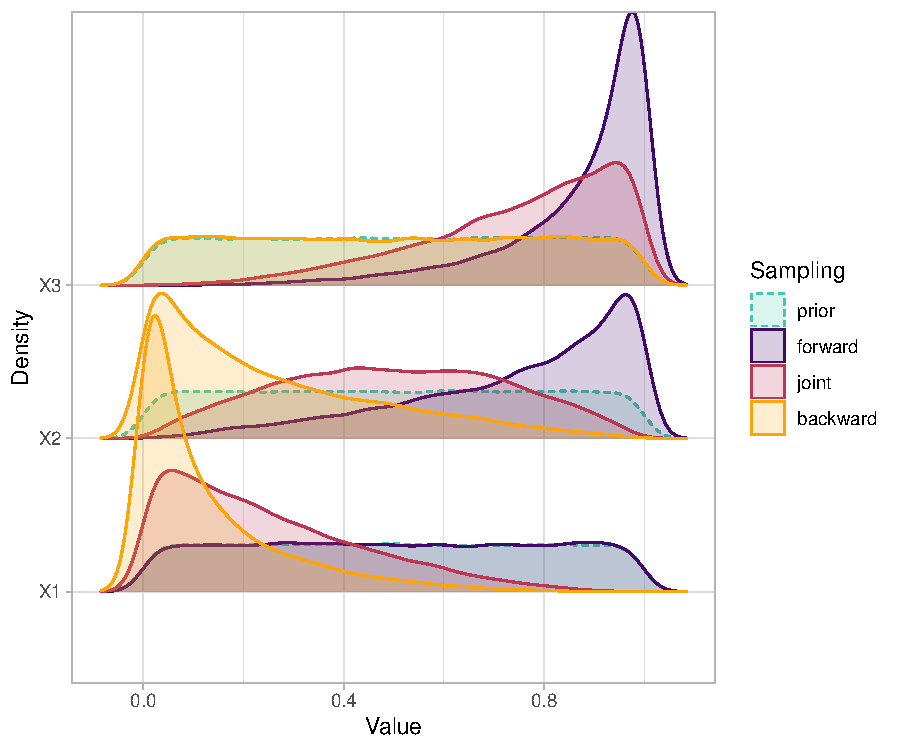
\includegraphics[scale=.67]{jsam.bias}
  \caption{Illustration of different sampling biases when enforcing $X_1 < X_2 < X_3$}
  \label{fig:jsam.bias}
  \floatfoot{Sampling method:
    \emph{joint:} sample $X_1$, $X_2$, $X_3$ simultaneously; then discard any samples failing $X_1 < X_2 < X_3$;
    \emph{forward:} sample $X_1$; then sample $X_2$ until $X_1 < X_2$; then sample $X_3$ until $X_2 < X_3$;
    \emph{backward:} sample $X_3$; then sample $X_2$ until $X_2 < X_3$; then sample $X_1$ until $X_1 < X_2$.}
\end{figure}
When sampling from the multivariate Gaussian distributions
during each IMIS step \cite{Raftery2010},
we attempted up to 1000 times per sample
to find a parameter set $\theta$ that satisfied all constraints;
if no such parameter set could be identified,
we set the weight of this $\theta$ to zero and continued.
%--------------------------------------------------------------------------------------------------
\paragraph{Likelihoods}
We defined the log likelihood $L_i$ of a given parameter set $\theta_i$ as
the sum of independent log likelihoods for each calibration target $T_j$:
\begin{equation}
  L_i = \sum\nolimits_{\,j} f_j \log p(T_j \mid \theta_i)
\end{equation}
where $f_j$ is a scale factor (usually 1) applied to target $T_j$
to increase or decrease its influence.
Any log likelihood which was beyond computational precision was replaced with
an arbitrarily large negative number: $-{10}^6$.
%--------------------------------------------------------------------------------------------------
\paragraph{Weights}
Due to the high number of calibration targets and thus high variance in log likelihoods,
IMIS weights defined per \cite{Raftery2010} exactly were usually degenerate,
having all-but-one near-zero values.
As such, our weight definitions used
the following transformation of log likelihoods
instead of actual likelihoods --- \ie $\exp(L)$:
\begin{equation}
  \tilde{L}_i = \frac{Q^{\,0.9}_{\,L}}{L_i}
\end{equation}
where $Q^{\,0.9}_{\,L}$ is the 90\% quantile of log likelihoods $L$.
Figure~\ref{fig:ll.tf} illustrates the shape of this transform \vs actual likelihoods,
for dummy log likelihoods uniformly distributed in log space $\in [-10^6,-10^1]$.
With this transformation: the 90\% quantile becomes 1,
a 10-fold higher $L$ becomes 10, and
a 10-fold lower $L$ becomes 0.1.
\begin{figure}[h]
  \centering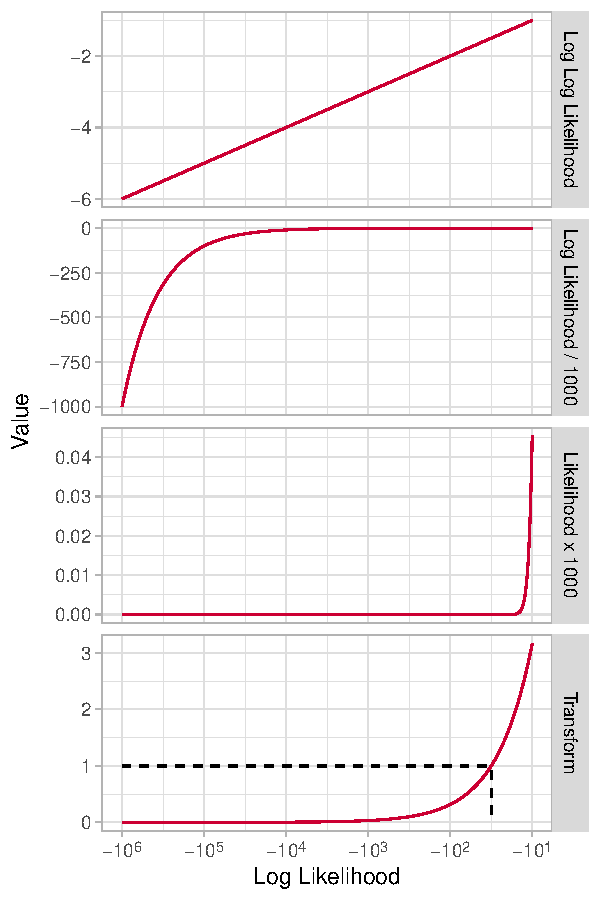
\includegraphics[scale=.67]{ll.tf}
  \caption{Shape of log likelihood transform used for IMIS weight definitions}
  \label{fig:ll.tf}
  \floatfoot{Dashed line indicates 90\% quantile of log likelihoods,
    corresponding to a value of 1 after transformation}
\end{figure}
These transformed log likelihoods $\tilde{L}$ were used instead of actual likelihoods
within the weight definitions for all stages:
after initial sampling, within each IMIS step, and for the final resampling.
%--------------------------------------------------------------------------------------------------
\paragraph{Iterations}
We ran 100 independent batches of the basic (without optimization) IMIS,
each with 1000 initial samples, 100 resamples per IMIS step, and 100 total IMIS steps
(1,100,000 total model runs),
from which we resampled 1000 posterior parameter sets (``model fits'') without replacement.
In the notation of \cite{Raftery2010}, we used 100 batches of: $N_0 = 1000, B = 100, J = 1000$.
We used batches to allow model fitting in parallel.
We did not use any stopping criterion,
but verified visually that log likelihoods plateaued within each batch.
